\setcounter{chapter}{3}
\chapter{偏微分方程式入門}
%
第1章で常微分方程式を学んだが,
これは未知関数に関する1変数の導関数しか含まない方程式のことを指す.
それに対し,偏微分方程式はその名前の通り,
偏導関数(つまり,未知関数は多変数関数)を含む方程式のことを指す.

自然現象を数式で表現しようとしたとき,
偏微分方程式に帰着することはよくある.
例えば,ある粒子が時刻$t$で3次元的な位置${\bf r} = \left(x,y,z\right)$に
存在する確率を$\psi$と表すことにすると,それは
$\psi\left(x,y,z,t\right)$のように4変数に依存しうるので,
その時間変化を表す方程式も偏微分方程式になる,というのは想像に難くない.
皆さんはこれから物質移動や熱の移動(熱伝導)について,
化学工学の講義で学んでいくことになる.
これらの現象は全て偏微分方程式によって表現されるので,これから化学工学を本格的に学んでいく上で,
偏微分方程式は外せない重要なトピックである.
実践的には,一般解を求めるよりも,問題設定に応じた初期条件や境界条件を満たす特殊解を求めることが重要となる.
そこで,この章では,偏微分方程式で表現される物理現象のいくつかを通して,特殊解を求める方法について学んでいくことにしよう.
時間の都合上,代表的な偏微分方程式の中でも数を絞って紹介せざるを得なかったが,
興味を持てた人は是非引き続き調べてみてほしい.
%そのため,他の章に比べて数学ではなく物理に関する解説が多めになっている.

%
\section{偏微分方程式での問題設定}
%
ここでは,2階の線形偏微分方程式を例にとって考えよう.
$x,~t$の2変数に依存する未知関数$\psi(x,t)$に対する線形偏微分方程式は,
一般に次のように表せる.
\begin{align}
A\dfrac{\partial^{2}\psi}{\partial x^{2}}+B\dfrac{\partial^{2}\psi}{\partial x\partial t}+C\dfrac{\partial^{2}\psi}{\partial t^{2}}+D\dfrac{\partial\psi}{\partial x}+E\dfrac{\partial\psi}{\partial t}+Fu & =G.
\end{align}
係数の大小関係に応じて,偏微分方程式を分類することが出来るが\footnote{放物型,双曲型,楕円型など.これらの名前の由来は,微分方程式の形と二次曲線の形の対比から来ている.},あまり気にしないでおくことにしよう.
以下の解説では,$x$は物質などの位置,$t$は時刻を表す変数と考えて読んで欲しい.
%
\subsection{初期条件}
%
常微分方程式の場合での初期条件というのは,1変数の未知関数$\psi(t)$の時刻$t=0$での値や,
導関数の$t=0$での値のことを指すのだった.
これに対し,偏微分方程式では時刻$t=0$での未知関数がとる関数が初期条件として与えられる.つまり,初期条件は
%
\begin{align}
  \psi\left(x,t=0\right) = f(x),
\end{align}
のような形で与えられる.
%
\subsection{境界条件}
%
注目している系が,領域$x_{\mathrm{min}}\leq x \leq x_{\mathrm{max}}$で定義されるものであったとする.
つまり,この系には端点が存在する.
偏微分方程式に対して,解やその導関数が端点でとるべき値などが指定されている場合,その条件のことを境界条件と呼ぶ.
以下で代表的な境界条件についてまとめておく.
\begin{itemize}
\item 
ディリクレ境界条件\\
境界条件として,解が端点でとるべき値が指定されているとき,
その条件のことをディリクレ境界条件と呼ぶ.
ディリクレ境界条件は,
\begin{align}
&\psi(x_{\mathrm{min}},t) = a_{0}, \\
&\psi(x_{\mathrm{max}},t) = a_{1},
\end{align}
のような形で与えられる.
%
\item
ノイマン境界条件\\
解の導関数がとるべき値が指定されているとき,
その条件のことをノイマン境界条件と呼ぶ.	
ノイマン境界条件は,
\begin{align}
& \dfrac{\partial }{\partial x}\psi(x,t)\biggr|_{x=x_{\mathrm{min}}} = a_{0}, \\ 
& \dfrac{\partial }{\partial x}\psi(x,t)\biggr|_{x=x_{\mathrm{max}}} = a_{1}, 
\end{align}
などのような形で境界条件が与えられる.
\end{itemize}
%
\section{変数分離法}
%
ここでは,例を通して変数分離法について学んでいくことにする.
偏微分方程式
\begin{align}
\dfrac{\partial}{\partial t}\psi\left(x,t\right)	=4\dfrac{\partial}{\partial x}\psi\left(x,t\right),
\end{align}
を考える.
ただし,初期条件は
\begin{align}
\psi\left(x,t=0\right)	=3e^{2x}+2e^{4x},
\end{align}
で与えられるとする.
変数分離法では,方程式を満たす解$\phi\left(x,t\right)$がそれぞれの変数のみに依存する関数$X\left(x\right),\,T\left(t \right)$の積で表せることを仮定する.つまり
\begin{align}
\psi\left(x,t\right)	=X\left(x\right)T\left(t\right),
\end{align}
の形を仮定して,初期条件や(後で触れる)境界条件を満たす特殊解を求めることになる.これを実際に与えられた方程式に代入してみると,
\begin{align}
&\dfrac{\partial}{\partial t}\left[X\left(x\right)T\left(t\right)\right]=4\dfrac{\partial}{\partial x}\left[X\left(x\right)T\left(t\right)\right],\notag \\
&\to X\left(x\right)\dfrac{d}{dt}T\left(t\right)=4T\left(t\right)\dfrac{d}{dx}X\left(x\right),\notag \\
&\to\dfrac{1}{T\left(t\right)}\dfrac{d}{dt}T\left(t\right)=\dfrac{4}{X\left(x\right)}\dfrac{d}{dx}X\left(x\right),
\end{align}
となる.最後の式をみると,左辺は$t$のみに依存する項,右辺は$x$のみに依存する項からなっている.上式が恒等的に成り立つためには,左辺,右辺ともに定数でなければならない.その定数を$\lambda$とおくと,
\begin{align}
\begin{cases}
\dfrac{1}{T\left(t\right)}\dfrac{d}{dt}T\left(t\right)=\lambda,\\[.4cm]
\dfrac{4}{X\left(x\right)}\dfrac{d}{dx}X\left(x\right)=\lambda,
\end{cases}
\end{align}
が得られる.それぞれの方程式は常微分方程式なので,第1章で学んだことが活きてくる.これらの特殊解は,
\begin{align}
\begin{cases}
T\left(t\right)=Ae^{\lambda t},\\
X\left(x\right)=Be^{\frac{\lambda}{4}x},
\end{cases}
\end{align}
である.従って,
\begin{align}
\psi\left(x,t\right)	=Ce^{\frac{\lambda}{4}x+\lambda t},
\end{align}
が解として考えられるが,この形では初期条件をどうやっても満たせない.今回の微分方程式を見ると,線形方程式であるから,解の1次結合も方程式の解となる.そこで,
\begin{align}
\psi\left(x,t\right)	=C_{1}e^{\frac{\lambda_{1}}{4}x+\lambda_{1}t}+C_{2}e^{\frac{\lambda_{2}}{4}x+\lambda_{2}t},
\end{align}
の形を考えてみる.すると,
\begin{align}
\psi\left(x,t=0\right)	=C_{1}e^{\frac{\lambda_{1}}{4}x}+C_{2}e^{\frac{\lambda_{2}}{4}x},
\end{align}
であるから,
\begin{align}
\lambda_{1}	=8,\,\lambda_{2}=16,\,C_{1}=3,\,C_{2}=2
\end{align}
とすれば,与えられた初期条件を満たす解が求められたことになる.
%
\section{拡散方程式}
%
$x$方向の1次元での物質密度の変化を考える.
時刻$t$,位置$x$での物質の密度を$\psi(x,t)$で表すことにする.
$\psi(x,t)$の時間変化を表す式として,次に示す拡散方程式がよく知られている.
%
\begin{align}
\dfrac{\partial}{\partial t}\psi\left(x,t\right) & =D\dfrac{\partial^{2}}{\partial x^{2}}\psi\left(x,t\right),\quad D>0.
\label{diffusion_eq_1d}
\end{align}
%
$D$は拡散係数と呼ばれ,物質が拡散する能力の度合いを表す.
%
\subsection{有限区間での拡散現象}
%

ここでは,物質が拡散する領域を区切った上で,この方程式の解を求めてみよう.
具体的には次のような境界条件を考える.
\begin{align}
\psi\left(x=0,t\right) & =\psi\left(x=L,t\right)=0.
\end{align}
この条件は,端点に到達した物質は,注目している区間から全て抜け出してしまう(つまり,区間内の物質量はその分だけ減少する),ということを反映している.
このあたりの解釈は物理的なものであって偏微分方程式の解法には関係しないので,もし難しければ今の段階ではスキップしても良い.
次に,初期条件として次式を考える.
\begin{align}
\psi\left(x,t=0\right) & =f\left(x\right).
\end{align}

ここまで問題を設定しておけば,あとは数学の問題だ.まず,$\psi(x,t)$として変数分離型の関数形を仮定する.
\begin{align}
\psi\left(x,t\right) & =X\left(x\right)T\left(t\right).
\end{align}
%
これを\Eq{diffusion_eq_1d}に代入すると,
%
\begin{align}
 & \dfrac{\partial}{\partial t}\left[X\left(x\right)T\left(t\right)\right]=D\dfrac{\partial^{2}}{\partial x^{2}}\left[X\left(x\right)T\left(t\right)\right],\notag\\
 & \to X\left(x\right)\dfrac{d}{dt}T\left(t\right)=DT\left(t\right)\dfrac{d^{2}}{dx^{2}}X\left(x\right),\notag\\
 & \to\dfrac{1}{D}\dfrac{1}{T\left(t\right)}\dfrac{d}{dt}T\left(t\right)=\dfrac{1}{X\left(x\right)}\dfrac{d^{2}}{dx^{2}}X\left(x\right).
\end{align}
左辺は$t$のみの関数,右辺は$x$のみの関数なので,両辺が恒等的に等しくなるためには定数である必要がある.
その定数を$\alpha$とおくと,
\begin{align}
 & \begin{cases}
\dfrac{1}{T\left(t\right)}\dfrac{d}{dt}T\left(t\right)=\alpha D,\\[.4cm]
\dfrac{1}{X\left(x\right)}\dfrac{d^{2}}{dx^{2}}X\left(x\right)=\alpha,
\end{cases}
\end{align}
である.第1式の解は,
\begin{align}
T\left(t\right) & =Ae^{\alpha Dt},
\end{align}
である.
$\alpha>0$の場合,$u\left(x,t\right)$は$t\to\infty$で無限大,つまり,粒子密度が無限大になるので,これは物理現象を表す解として不適切である.従って,$\alpha<0$である.ここでは,$\alpha=-\lambda^{2}$と表すことにする.すると,
\begin{align}
T\left(t\right) & =A\exp\left(-\lambda^{2}Dt\right),\\
X\left(x\right) & =B\cos\left(\lambda x\right)+C\sin\left(\lambda x\right),
\end{align}
なので,
\begin{align}
\psi\left(x,t\right) & =AB\exp\left(-\lambda^{2}Dt\right)\cos\left(\lambda x\right)+AC\exp\left(-\lambda^{2}Dt\right)\sin\left(\lambda x\right).
\end{align}
境界条件について考えよう.
$x=0$での境界条件より,
\begin{align}
\psi\left(0,t \right) & =AB\exp\left(-\lambda^{2}Dt\right)=0
\end{align}
$A=0$の場合は$\psi=0$になってしまうので,$B=0$である.従って,
\begin{align}
\psi\left(x,t\right) & =AC\exp\left(-\lambda^{2}Dt\right)\sin\left(\lambda x\right),
\end{align}
である.次に,$x=L$での境界条件より,
\begin{align}
\psi\left(L,t\right) & =AC\exp\left(-\lambda^{2}Dt\right)\sin\left(\lambda L\right)=0
\end{align}
$C=0$では,$\psi=0$になってしまうので,この条件からは
\begin{align}
 & \sin\left(\lambda L\right)=0,\\
 & \to\lambda_{n}=\dfrac{\pi n}{L},\quad n=1,2,\cdots
\end{align}
が得られるので,解の形として
\begin{align}
\psi\left(x,t\right) & =\sum_{n=1}^{\infty}C_{n}\exp\left(-\lambda_{n}^{2}Dt\right)\sin\left(\lambda_{n}x\right),
\end{align}
が得られる.初期条件から,
\begin{align}
\psi\left(x,t=0\right) & =\sum_{n=1}^{\infty}C_{n}\sin\left(\lambda_{n}x\right)=f\left(x\right),
\end{align}
である.
これは$f\left(x\right)$をフーリエ正弦級数展開していることに他ならない.つまり,初期条件で与えられた関数$f\left(x\right)$をフーリエ正弦級数展開して,各$\lambda_{n}~(=\pi n/L)$ごとの展開係数$C_{n}$を決定すれば,
初期条件を満たす偏微分方程式の解が得られたことになる.
%
\subsection{無限区間での拡散現象(1次元)}
%
一つ前の例では,有限区間での拡散方程式の解を求めた.
その際,初期条件をフーリエ級数展開することで,条件を満たす方程式の解が求められる,というのがミソだった.
この方法は注目している系が有限区間で,初期条件で与えられる関数を周期関数に拡張することが
出来たのであって,無限区間($-\infty < x < \infty$)では同じ方法は使えない.
このような場合は非周期関数を扱えるフーリエ変換を用いると良い.

まず,問題設定をしておこう.
拡散方程式
\begin{align}
 \dfrac{\partial}{\partial t}\psi\left(x,t\right) & =D\dfrac{\partial^{2}}{\partial x^{2}}\psi\left(x,t\right),
\end{align}
に対して,初期条件
\begin{align}
\psi\left(x,t=0\right) & = \psi_{0}(x), 
\end{align}
を課しておく.
$\psi(x,t)$の$x$に対するフーリエ変換を次式で定義する.
\begin{align}
  \hat{\psi}(k,t) = \int_{0}^{\infty}dx\,e^{-ikx}\psi(x,t).
\end{align}
$\psi_{0}(x)$についても,同様にしてフーリエ変換$\hat{\psi}_{0}(k)$を定義しておく.
次に,拡散方程式のフーリエ変換を行うが,微分のフーリエ変換の公式(\Eq{deriv_fourier})
\begin{align}
 \mathcal{F}\left[\dfrac{d^2}{dx^2}\psi(x,t)\right] = -k^2 \hat{\psi}(k,t), 
\end{align}
を用いると良い.変換後の拡散方程式は,
\begin{align}
  \dfrac{\partial}{\partial t}\hat{\psi}(k,t) = -k^{2}D\hat{\psi}(k,t), 
\end{align}
であり,$t$に関する常微分方程式である.
これを解くのは簡単であり,解は
\begin{align}
 \hat{\psi}(k,t) = \exp\left[-k^2 D t\right]\hat{\psi}_{0}(k), 
\end{align}
で与えられる.フーリエ逆変換を実行できれば,偏微分方程式の解が得られたことになる.
\begin{align}
\psi\left(x,t\right) & =\dfrac{1}{2\pi}\int_{-\infty}^{\infty}dk\,e^{ikx}\exp\left[-k^{2}Dt\right]\hat{\psi}_{0}\left(k\right)\notag\\
 & =\dfrac{1}{2\pi}\int_{-\infty}^{\infty}dk\,e^{ikx}\exp\left[-k^{2}Dt\right]\int_{-\infty}^{\infty}dx^{\prime}\,e^{-ikx^{\prime}}\psi_{0}\left(x^{\prime}\right)\notag\\
 & =\dfrac{1}{2\pi}\int_{-\infty}^{\infty}dx^{\prime}\,\psi_{0}\left(x^{\prime}\right)\int_{-\infty}^{\infty}dk\,\exp\left[ik\left(x-x^{\prime}\right)-k^{2}Dt\right]\notag\\
 & =\dfrac{1}{2\pi}\int_{-\infty}^{\infty}dx^{\prime}\,\psi_{0}\left(x^{\prime}\right)\int_{-\infty}^{\infty}dk\,\exp\left[-Dt\left(k-\dfrac{i}{2Dt}\left(x-x^{\prime}\right)\right)^{2}-\dfrac{\left(x-x^{\prime}\right)^{2}}{4Dt}\right]\notag\\
 & =\dfrac{1}{2\pi}\int_{-\infty}^{\infty}dx^{\prime}\,\psi_{0}\left(x^{\prime}\right)\sqrt{\dfrac{\pi}{Dt}}\exp\left[-\dfrac{\left(x-x^{\prime}\right)^{2}}{4Dt}\right]\notag\\
 & =\dfrac{1}{\sqrt{4\pi Dt}}\int_{-\infty}^{\infty}dx^{\prime}\,\psi_{0}\left(x^{\prime}\right)\exp\left[-\dfrac{\left(x-x^{\prime}\right)^{2}}{4Dt}\right]
\end{align}

\subsection{無限区間での拡散現象(3次元)}
%
せっかくなので,3次元空間${\bf r}=(x,y,z)$での拡散について考えてみよう.
1次元とほぼ全く同じ手続きで解を求められる.

3次元の場合の拡散方程式は次式である.
%
\begin{align}
 \dfrac{\partial}{\partial t}\psi\left({\bf r},t\right) & =D\nabla^{2}\psi\left({\bf r},t\right)\notag\\
 & =D\left(\dfrac{\partial^{2}}{\partial x^{2}}\psi\left({\bf r},t\right)+\dfrac{\partial^{2}}{\partial y^{2}}\psi\left({\bf r},t\right)+\dfrac{\partial^{2}}{\partial z^{2}}\psi\left({\bf r},t\right)\right).
\end{align}
%
ちなみに,1行目の$\nabla^{2}$はラプラシアンと呼ばれる演算子で,
\begin{align}
\nabla^{2} & =\dfrac{\partial^{2}}{\partial x^{2}}+\dfrac{\partial^{2}}{\partial y^{2}}+\dfrac{\partial^{2}}{\partial z^{2}},
\end{align}
で定義される.
%

3次元空間でのフーリエ変換(${\bf r}\to {\bf k}$)は
\begin{align}
\hat{\psi}\left({\bf k},t\right) & =\int d{\bf r}\,e^{-i{\bf k}\cdot{\bf r}}\psi\left({\bf r},t\right)\notag\\
 & =\int_{-\infty}^{\infty}\int_{-\infty}^{\infty}\int_{-\infty}^{\infty}dxdydz\,\exp\left[-ik_{x}x-ik_{y}y-ik_{z}z\right]\psi\left(x,y,z,t\right),
\end{align}
である.
拡散方程式のフーリエ変換を計算してみよう.
1次元の場合よりも難しそうに思うかもしれないが,ベクトル表示${\bf r}$, ${\bf k}$を成分表示に直してみると,実は1次元の場合と同じである.
とは言え,
いきなりそんなこと言われても困るかもしれないので,くどいくらい途中の式変形を示すことにする\footnote{3次元拡散方程式の解を導くのに,こんなに長ったらしく式変形を書いている書籍は見たことがないので,もしかすると,余計なお節介なレベルなのかもしれないが,
その場合は適宜読み飛ばして欲しい.}.
まず,フーリエ変換の定義から,次式のように式変形する.
\begin{align}
\dfrac{\partial}{\partial t}\hat{\psi}\left({\bf k},t\right) & =D\int d{\bf r}\,e^{-i{\bf k}\cdot{\bf r}}\,\nabla^{2}\psi\left({\bf r},t\right)\notag\\
 & =D\int_{-\infty}^{\infty}\int_{-\infty}^{\infty}\int_{-\infty}^{\infty}dxdydz\,\exp\left[-ik_{x}x-ik_{y}y-ik_{z}z\right]\notag\\
 & \qquad\times\left(\dfrac{\partial^{2}}{\partial x^{2}}\psi\left(x,y,z,t\right)+\dfrac{\partial^{2}}{\partial y^{2}}\psi\left(x,y,z,t\right)+\dfrac{\partial^{2}}{\partial z^{2}}\psi\left(x,y,z,t\right)\right)\notag\\
 & =D\int_{-\infty}^{\infty}\int_{-\infty}^{\infty}dydz\,\exp\left[-ik_{y}y-ik_{z}z\right]\int_{-\infty}^{\infty}dx\,\exp\left[-ik_{x}x\right]\dfrac{\partial^{2}}{\partial x^{2}}\psi\left(x,y,z,t\right)\notag\\
 & \quad+D\int_{-\infty}^{\infty}\int_{-\infty}^{\infty}dxdz\,\exp\left[-ik_{x}x-ik_{z}z\right]\int_{-\infty}^{\infty}dy\,\exp\left[-ik_{y}y\right]\dfrac{\partial^{2}}{\partial y^{2}}\psi\left(x,y,z,t\right)\notag\\
 & \quad+D\int_{-\infty}^{\infty}\int_{-\infty}^{\infty}dxdy\,\exp\left[-ik_{x}x-ik_{y}y\right]\int_{-\infty}^{\infty}dz\,\exp\left[-ik_{z}z\right]\dfrac{\partial^{2}}{\partial z^{2}}\psi\left(x,y,z,t\right).
\end{align}
$\psi\left({\bf r},t\right)$の$\alpha$成分($\alpha=x,y,z$)のみをフーリエ変換したものを$\hat{\psi}_{\alpha}$と表すことにすると,上式は
\begin{align}
 \dfrac{\partial}{\partial t}\hat{\psi}\left({\bf k},t\right) & =D\int_{-\infty}^{\infty}\int_{-\infty}^{\infty}dydz\,\exp\left[-ik_{y}y-ik_{z}z\right]\left(-k_{x}^{2}\hat{\psi}_{x}\left(k_{x},y,z,t\right)\right)\notag\\
 & \quad+D\int_{-\infty}^{\infty}\int_{-\infty}^{\infty}dxdz\,\exp\left[-ik_{x}x-ik_{z}z\right]\left(-k_{y}^{2}\hat{\psi}_{y}\left(x,k_{y},z,t\right)\right)\notag\\
 & \quad+D\int_{-\infty}^{\infty}\int_{-\infty}^{\infty}dxdy\,\exp\left[-ik_{x}x-ik_{y}y\right]\left(-k_{z}^{2}\hat{\psi}_{z}\left(x,y,k_{z},t\right)\right).
\end{align}
残りの積分も実行することで,
\begin{align}
 \dfrac{\partial}{\partial t}\hat{\psi}\left({\bf k},t\right) & =-k_{x}^{2}D\hat{\psi}\left({\bf k},t\right)-k_{y}^{2}D\hat{\psi}\left({\bf k},t\right)-k_{z}^{2}D\hat{\psi}\left({\bf k},t\right)\notag\\
 & =-k^{2}D\hat{\psi}\left({\bf k},t\right),
\end{align}
を得る.
この$t$に関する常微分方程式の解は
\begin{align}
 \hat{\psi}({\bf k},t) = \exp\left[-k^2 D t\right] \hat{\psi}_{0}({\bf k}), 
\end{align}
である.逆変換すれば,実空間でちゃんと目的の解が得られたことになる.
逆変換の場合も,成分表示で書いて考えてみると良い.
\begin{align}
\psi\left({\bf r},t\right) & =\dfrac{1}{\left(2\pi^{3}\right)}\int d{\bf k}\,e^{i{\bf k}\cdot{\bf r}}\exp\left[-k^{2}Dt\right]\hat{\psi_{0}}\left({\bf k}\right)\notag\\
 & =\dfrac{1}{\left(2\pi\right)^{3}}\int_{-\infty}^{\infty}dk_{x}\int_{-\infty}^{\infty}dk_{y}\int_{-\infty}^{\infty}dk_{z}\,\exp\left[ik_{x}x+ik_{y}y+ik_{z}z\right]\exp\left[-\left(k_{x}^{2}+k_{y}^{2}+k_{z}^{2}\right)Dt\right]\notag\\
 & \qquad\times\int_{-\infty}^{\infty}dx\int_{-\infty}^{\infty}dy\int_{-\infty}^{\infty}dz\,\exp\left[-ik_{x}x^{\prime}-ik_{y}y^{\prime}-ik_{z}z^{\prime}\right]\psi_{0}\left(x^{\prime},y^{\prime},z^{\prime}\right)\notag\\
 & =\dfrac{1}{\left(2\pi\right)^{3}}\int_{-\infty}^{\infty}dx\int_{-\infty}^{\infty}dy\int_{-\infty}^{\infty}dz\,\psi\left(x^{\prime},y^{\prime},z^{\prime}\right)\notag\\
 & \qquad\times\int_{-\infty}^{\infty}dk_{x}\,\exp\left[-Dt\left(k_{x}-\dfrac{i}{2Dt}\left(x-x^{\prime}\right)\right)^{2}\right]\exp\left[-\dfrac{\left(x-x^{\prime}\right)^{2}}{4Dt}\right]\notag\\
 & \qquad\times\int_{-\infty}^{\infty}dk_{y}\,\exp\left[-Dt\left(k_{y}-\dfrac{i}{2Dt}\left(y-y^{\prime}\right)\right)^{2}\right]\exp\left[-\dfrac{\left(y-y^{\prime}\right)^{2}}{4Dt}\right]\notag\\
 & \qquad\times\int_{-\infty}^{\infty}dk_{z}\,\exp\left[-Dt\left(k_{z}-\dfrac{i}{2Dt}\left(z-z^{\prime}\right)\right)^{2}\right]\exp\left[-\dfrac{\left(z-z^{\prime}\right)^{2}}{4Dt}\right]\notag\\
 & =\dfrac{1}{\left(4\pi Dt\right)^{3/2}}\int d{\bf r}^{\prime}\,\psi_{0}\left({\bf r}^{\prime}\right)\exp\left[-\dfrac{\left|{\bf r}-{\bf r}^{\prime}\right|^{2}}{4Dt}\right].
\end{align}
%

教科書などにはよく,初期条件が
\begin{align}
  \psi_{0}\left({\bf r}\right) = \delta \left(\bf r\right),
\end{align}
の場合の結果が紹介されているが,これを求めた解に代入すると,
\begin{align}
\psi\left({\bf r},t\right) & =\dfrac{1}{\left(4\pi Dt\right)^{3/2}}\exp\left[-\dfrac{1}{4Dt}\left|{\bf r}\right|^{2}\right],
\end{align}
%
%\begin{wrapfigure}[8]{r}{6cm}
\begin{figure}[htbp]
 \centering
 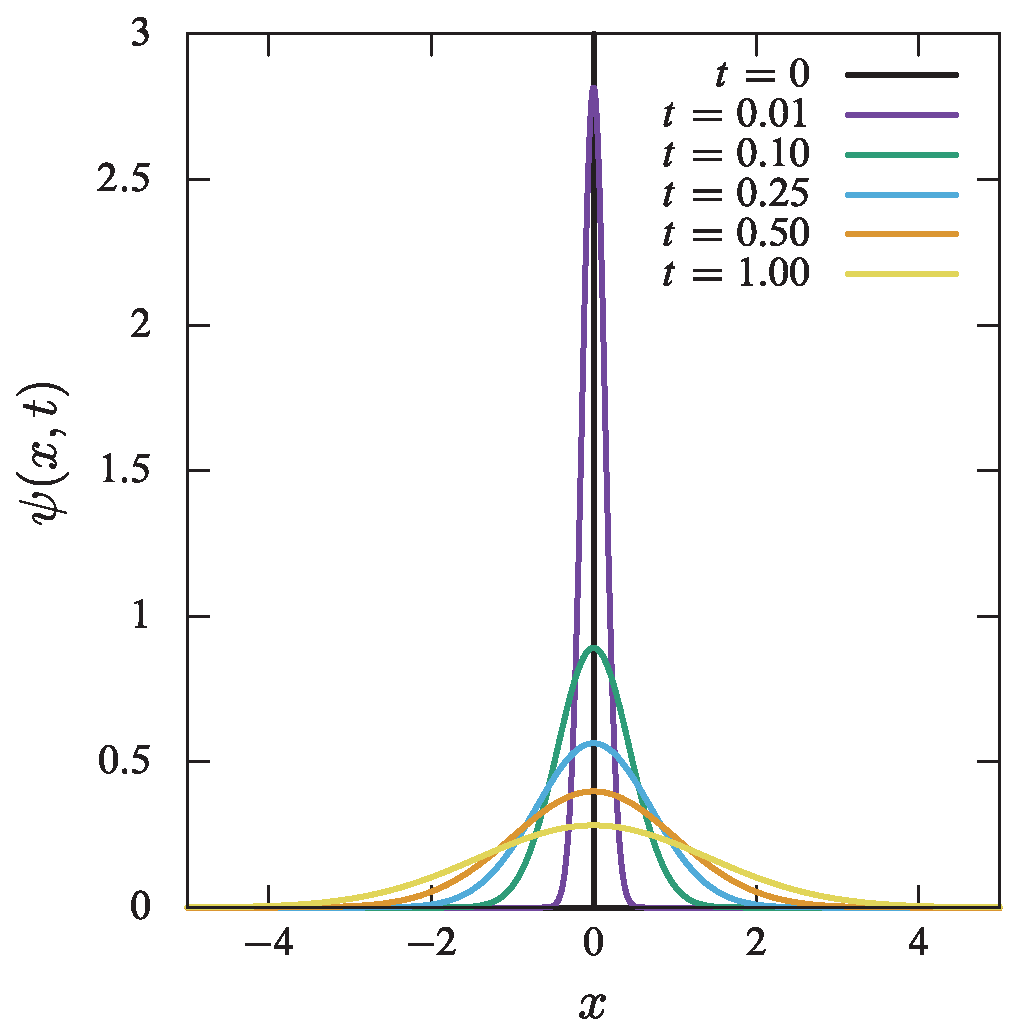
\includegraphics[width=0.5\linewidth]{/Users/kasa/Dropbox/GitHub/lectures/osaka-u/2021/kaenI/chap04_pd/figures/diff.eps} 
\end{figure}
%\end{wrapfigure}
となる.時刻$t=0$で特定の位置(${\bf r}={\bf 0}$)に局在していた物質が,
Gauss関数の形で空間的に広がっていくのが,解の形を見れば分かる.
1次元の場合の拡散方程式の解を次図に示しておく.

%
\section{波動方程式}
%
媒質を伝播する波の時間変化は,波動方程式と呼ばれる偏微分方程式によって記述される.
ここでは,まず簡単な例を通して波動方程式を示した後,
無限に広がる媒質の中での波の時間変化について見てみよう.
%
\subsection{波動方程式の導出}
%
\begin{figure}[htbp]
%\begin{wrapfigure}{r}{6cm}
  \centering
  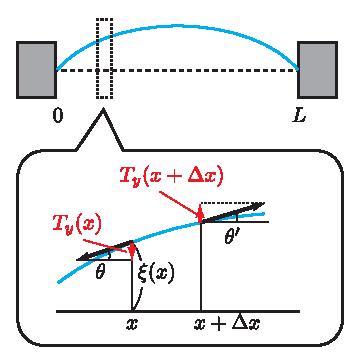
\includegraphics[width=0.5\linewidth]{/Users/kasa/Dropbox/GitHub/lectures/osaka-u/2021/kaenI/chap04_pd/figures/string.eps} 
%\end{wrapfigure}
\end{figure}
弦楽器のように,両端を固定された弦の振動について考えてみよう.
上図のように両端を固定された長さ$L$の弦を考える.
また,弦の単位長さあたりの質量密度を$\rho$,弦に働く張力を$T$とする.
弦の微小部分($x\sim x+\Delta x$)に注目すると,
その部分の質量$m$は,
\begin{align}
  m = \rho \Delta x, 
\end{align}
である.そして,位置$x$での弦の変位を$\xi(x)$とすると,微小部分の変位に関する運動方程式は,
Newtonの運動方程式から
\begin{align}
 F_{y} &= m\dfrac{\partial^{2}\xi(x)}{\partial t^2} \notag \\
       &= \rho \Delta x \dfrac{\partial^{2}\xi(x)}{\partial t^2}, \label{Newton_eq_string} 
\end{align}
と表せる.ここで,$F_{y}$は弦の微小部位にかかる力の変位方向($y$)の成分である.
張力は弦の接線方向に働くので,$x$軸の方向と弦のなす角によって,張力の$y$成分$T_{y}$が決まる.
図の幾何的考察から,
\begin{align}
  &T_{y}(x)    = -T \sin \theta, \\
  &T_{y}(x+\Delta x) =  T \sin \theta^{\prime},  
\end{align}
と表せることが分かる.従って,
\begin{align}
  F_{y} &= T_{y}(x+\Delta x)+ T_{y}(x)  \notag \\
        &= T\left(\sin\theta^{\prime}-\sin\theta\right), \label{force_string}
\end{align}
である.変位が小さい場合は,$\theta,~\theta^{\prime}$も小さいので,
\begin{align}
  &\sin\theta = \theta - \dfrac{1}{3!}\theta^{3} + \cdots \simeq \theta, \\
  &\cos\theta = 1 - \dfrac{1}{2!}\theta^2 + \cdots \simeq 1, 
\end{align}
と近似出来るので,
\begin{align}
  \dfrac{\partial \xi (x)}{\partial x} = \tan \theta  = \dfrac{\sin \theta}{\cos \theta} \simeq \sin \theta,
\end{align}
と表しても良い.これを\Eq{force_string}に代入することで,
\begin{align}
 F_y & =  T\left(\dfrac{\partial \xi }{\partial x}\biggr|_{x=x+\Delta x} - \dfrac{\partial \xi}{\partial x}\biggr|_{x=x}\right) \notag \\
     & = T\dfrac{\partial^2 \xi}{\partial x^2} \Delta x
\end{align}
を得る.従って,運動方程式\Eq{Newton_eq_string}から,
\begin{align}
  \dfrac{\partial^2 \xi}{\partial t^2} = v^{2} \dfrac{\partial^2 \xi}{\partial x^2}, \label{wave_eq} 
\end{align}
となる.ただし,
\begin{align}
  v = \sqrt{\dfrac{T}{\rho}},
\end{align}
とおいた.\Eq{wave_eq}は波動方程式と呼ばれ,媒質を伝わる振動現象(波動)を記述する上での基礎となる.
注目している現象によって,$v$の表式は異なるが,波動方程式の形自体は共通している.
今回は端点を固定した場合で波動方程式を示したが,自由端の場合も同じ形の偏微分方程式になる.
また,$v$が波の進行速度を表していることが,より詳細な考察から分かる.
%
\subsection{無限に広がる媒質中での波}
%
無限に広がる媒質(無限区間,$-\infty < x < \infty$)を伝わる
波の時間変化$u(x,t)$について見ていこう.$u(x,t)$として何を想像しても良いが,
先程の例と同じで,弦(ただし無限に長い)の変位のようなものを考えておこう.
その基礎方程式として,波動方程式
\begin{align}
 \dfrac{\partial^{2}}{\partial t^{2}}u\left(x,t\right) & =v^{2}\dfrac{\partial}{\partial x^{2}}u\left(x,t\right),
\end{align}
を考える.ここでは,初期条件として
\begin{align}
  &u(x,t=0) = f(x), \\
  &\dfrac{\partial}{\partial t}u(x,t)\biggr|_{t=0} = 0,
\end{align}
を与えておく.

まず,$u(x,t)$と$f(x)$のフーリエ変換をそれぞれ,
\begin{align}
 & \hat{u}\left(k,t\right)=\int_{-\infty}^{\infty}dx\,e^{-ikx}u\left(x,t\right),\\
 & \hat{f}\left(k\right)=\int_{-\infty}^{\infty}dx\,e^{-ikx}f\left(x\right), 
\end{align}
で定義する.

波動方程式のフーリエ変換は次式である.
\begin{align}
\dfrac{\partial^{2}}{\partial t^{2}}\hat{u}\left(k,t\right) & =-v^{2}k^{2}\hat{u}\left(k,t\right).
\end{align}
この$t$に関する常微分方程式の解は
\begin{align}
  \hat{u}(k,t) = A(k)\cos(vkt) + B(k)\sin(vkt), 
\end{align}
である.初期条件を考えると,
\begin{align}
  A(k) = \hat{f}(k), \quad B(k) = 0,
\end{align}
つまり,
\begin{align}
  \hat{u}(k,t) = \hat{f}(k)\cos(vkt), 
\end{align}
である.次は上式のフーリエ逆変換を計算するわけだが,まず$\cos(vkt)$の逆変換を計算しておこう.
\begin{align}
\mathcal{F}^{-1}\left[\cos\left(vkt\right)\right] & =\dfrac{1}{2\pi}\int_{-\infty}^{\infty}dk\,e^{ikx}\cos\left(vkt\right)\notag\\
 & =\dfrac{1}{2\pi}\int_{-\infty}^{\infty}dk\,e^{ikx}\dfrac{e^{ivkt}+e^{-ivkt}}{2}\notag\\
 & =\dfrac{1}{2}\left(\dfrac{1}{2\pi}\int_{-\infty}^{\infty}dk\,e^{ik\left(x+vt\right)}+\dfrac{1}{2\pi}\int_{-\infty}^{\infty}dk\,e^{ik\left(x-vt\right)}\right)\notag\\
 & =\dfrac{1}{2}\left(\delta\left(x+vt\right)+\delta\left(x-vt\right)\right).
\end{align}
上式の導出の際には,第3章で学んだデルタ関数の表式\Eq{deltafunc_fourier}
\begin{align}
 \delta (x) = \dfrac{1}{2\pi}\int_{-\infty}^{\infty}dk\,e^{ikx}, 
\end{align}
を用いた.
$\hat{u}(k,t)$は$\hat{f}(k)$と$\cos(vkt)$の積になっているが,これは畳み込み積分のフーリエ変換の公式\Eq{fourier_convolution}を逆から見れば,
\begin{align}
 u\left(x,t\right) & =\int_{-\infty}^{\infty}dy\,f\left(y\right)\dfrac{1}{2}\left(\delta\left(x-y+vt\right)+\delta\left(x-y-vt\right)\right)\notag\\
 & =\dfrac{1}{2}\left(f\left(x-vt\right)+f\left(x+vt\right)\right),
\end{align}
とできる.

この解は$t=0$で$f(x)$の形をとっていた状態が,半分の高さで左右に分かれて伝わっていくことを意味している(次図参照).この解のことをダランベールの解と呼ぶ.
%\newpage
\begin{figure}[htbp]
 \centering
 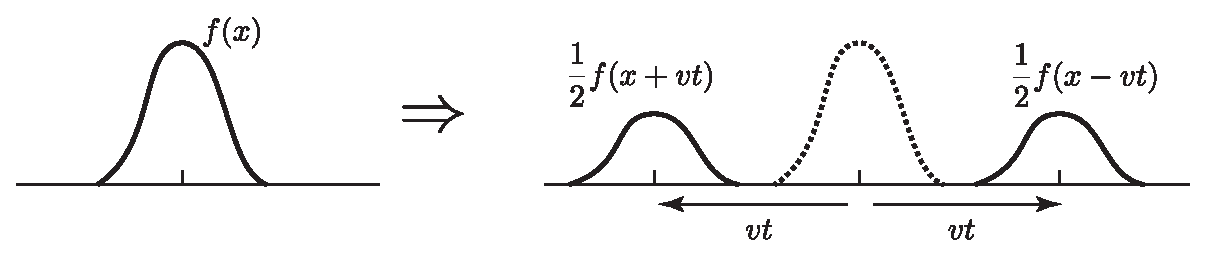
\includegraphics[width=0.8\linewidth]{/Users/kasa/Dropbox/GitHub/lectures/osaka-u/2021/kaenI/chap04_pd/figures/wave_eq_sol01.eps} 
\end{figure}